% Options for packages loaded elsewhere
\PassOptionsToPackage{unicode}{hyperref}
\PassOptionsToPackage{hyphens}{url}
%
\documentclass[
]{book}
\usepackage{amsmath,amssymb}
\usepackage{lmodern}
\usepackage{iftex}
\ifPDFTeX
  \usepackage[T1]{fontenc}
  \usepackage[utf8]{inputenc}
  \usepackage{textcomp} % provide euro and other symbols
\else % if luatex or xetex
  \usepackage{unicode-math}
  \defaultfontfeatures{Scale=MatchLowercase}
  \defaultfontfeatures[\rmfamily]{Ligatures=TeX,Scale=1}
\fi
% Use upquote if available, for straight quotes in verbatim environments
\IfFileExists{upquote.sty}{\usepackage{upquote}}{}
\IfFileExists{microtype.sty}{% use microtype if available
  \usepackage[]{microtype}
  \UseMicrotypeSet[protrusion]{basicmath} % disable protrusion for tt fonts
}{}
\makeatletter
\@ifundefined{KOMAClassName}{% if non-KOMA class
  \IfFileExists{parskip.sty}{%
    \usepackage{parskip}
  }{% else
    \setlength{\parindent}{0pt}
    \setlength{\parskip}{6pt plus 2pt minus 1pt}}
}{% if KOMA class
  \KOMAoptions{parskip=half}}
\makeatother
\usepackage{xcolor}
\usepackage{color}
\usepackage{fancyvrb}
\newcommand{\VerbBar}{|}
\newcommand{\VERB}{\Verb[commandchars=\\\{\}]}
\DefineVerbatimEnvironment{Highlighting}{Verbatim}{commandchars=\\\{\}}
% Add ',fontsize=\small' for more characters per line
\usepackage{framed}
\definecolor{shadecolor}{RGB}{248,248,248}
\newenvironment{Shaded}{\begin{snugshade}}{\end{snugshade}}
\newcommand{\AlertTok}[1]{\textcolor[rgb]{0.94,0.16,0.16}{#1}}
\newcommand{\AnnotationTok}[1]{\textcolor[rgb]{0.56,0.35,0.01}{\textbf{\textit{#1}}}}
\newcommand{\AttributeTok}[1]{\textcolor[rgb]{0.77,0.63,0.00}{#1}}
\newcommand{\BaseNTok}[1]{\textcolor[rgb]{0.00,0.00,0.81}{#1}}
\newcommand{\BuiltInTok}[1]{#1}
\newcommand{\CharTok}[1]{\textcolor[rgb]{0.31,0.60,0.02}{#1}}
\newcommand{\CommentTok}[1]{\textcolor[rgb]{0.56,0.35,0.01}{\textit{#1}}}
\newcommand{\CommentVarTok}[1]{\textcolor[rgb]{0.56,0.35,0.01}{\textbf{\textit{#1}}}}
\newcommand{\ConstantTok}[1]{\textcolor[rgb]{0.00,0.00,0.00}{#1}}
\newcommand{\ControlFlowTok}[1]{\textcolor[rgb]{0.13,0.29,0.53}{\textbf{#1}}}
\newcommand{\DataTypeTok}[1]{\textcolor[rgb]{0.13,0.29,0.53}{#1}}
\newcommand{\DecValTok}[1]{\textcolor[rgb]{0.00,0.00,0.81}{#1}}
\newcommand{\DocumentationTok}[1]{\textcolor[rgb]{0.56,0.35,0.01}{\textbf{\textit{#1}}}}
\newcommand{\ErrorTok}[1]{\textcolor[rgb]{0.64,0.00,0.00}{\textbf{#1}}}
\newcommand{\ExtensionTok}[1]{#1}
\newcommand{\FloatTok}[1]{\textcolor[rgb]{0.00,0.00,0.81}{#1}}
\newcommand{\FunctionTok}[1]{\textcolor[rgb]{0.00,0.00,0.00}{#1}}
\newcommand{\ImportTok}[1]{#1}
\newcommand{\InformationTok}[1]{\textcolor[rgb]{0.56,0.35,0.01}{\textbf{\textit{#1}}}}
\newcommand{\KeywordTok}[1]{\textcolor[rgb]{0.13,0.29,0.53}{\textbf{#1}}}
\newcommand{\NormalTok}[1]{#1}
\newcommand{\OperatorTok}[1]{\textcolor[rgb]{0.81,0.36,0.00}{\textbf{#1}}}
\newcommand{\OtherTok}[1]{\textcolor[rgb]{0.56,0.35,0.01}{#1}}
\newcommand{\PreprocessorTok}[1]{\textcolor[rgb]{0.56,0.35,0.01}{\textit{#1}}}
\newcommand{\RegionMarkerTok}[1]{#1}
\newcommand{\SpecialCharTok}[1]{\textcolor[rgb]{0.00,0.00,0.00}{#1}}
\newcommand{\SpecialStringTok}[1]{\textcolor[rgb]{0.31,0.60,0.02}{#1}}
\newcommand{\StringTok}[1]{\textcolor[rgb]{0.31,0.60,0.02}{#1}}
\newcommand{\VariableTok}[1]{\textcolor[rgb]{0.00,0.00,0.00}{#1}}
\newcommand{\VerbatimStringTok}[1]{\textcolor[rgb]{0.31,0.60,0.02}{#1}}
\newcommand{\WarningTok}[1]{\textcolor[rgb]{0.56,0.35,0.01}{\textbf{\textit{#1}}}}
\usepackage{longtable,booktabs,array}
\usepackage{calc} % for calculating minipage widths
% Correct order of tables after \paragraph or \subparagraph
\usepackage{etoolbox}
\makeatletter
\patchcmd\longtable{\par}{\if@noskipsec\mbox{}\fi\par}{}{}
\makeatother
% Allow footnotes in longtable head/foot
\IfFileExists{footnotehyper.sty}{\usepackage{footnotehyper}}{\usepackage{footnote}}
\makesavenoteenv{longtable}
\usepackage{graphicx}
\makeatletter
\def\maxwidth{\ifdim\Gin@nat@width>\linewidth\linewidth\else\Gin@nat@width\fi}
\def\maxheight{\ifdim\Gin@nat@height>\textheight\textheight\else\Gin@nat@height\fi}
\makeatother
% Scale images if necessary, so that they will not overflow the page
% margins by default, and it is still possible to overwrite the defaults
% using explicit options in \includegraphics[width, height, ...]{}
\setkeys{Gin}{width=\maxwidth,height=\maxheight,keepaspectratio}
% Set default figure placement to htbp
\makeatletter
\def\fps@figure{htbp}
\makeatother
\setlength{\emergencystretch}{3em} % prevent overfull lines
\providecommand{\tightlist}{%
  \setlength{\itemsep}{0pt}\setlength{\parskip}{0pt}}
\setcounter{secnumdepth}{5}
\usepackage{booktabs}
\ifLuaTeX
  \usepackage{selnolig}  % disable illegal ligatures
\fi
\usepackage[]{natbib}
\bibliographystyle{apalike}
\IfFileExists{bookmark.sty}{\usepackage{bookmark}}{\usepackage{hyperref}}
\IfFileExists{xurl.sty}{\usepackage{xurl}}{} % add URL line breaks if available
\urlstyle{same} % disable monospaced font for URLs
\hypersetup{
  pdftitle={Quantitative Methods - R Cookbook},
  pdfauthor={Subash Parajuli},
  hidelinks,
  pdfcreator={LaTeX via pandoc}}

\title{Quantitative Methods - R Cookbook}
\author{Subash Parajuli}
\date{2023-04-04}

\begin{document}
\maketitle

{
\setcounter{tocdepth}{1}
\tableofcontents
}
\hypertarget{welcome}{%
\chapter*{Welcome}\label{welcome}}
\addcontentsline{toc}{chapter}{Welcome}

Welcome to Quantitative Methods - R Cookbook. This cookbook covers practical worked out examples which you can easily apply to your dataset and also includes a discussion on how the recipe is working. We will cover descriptive and basic inferential statistics, including graphs, frequency distributions, central tendency, dispersion, probability, hypothesis testing, tests of mean differences, correlation and simple regression, and chi-square tests. This cookbook is designed to facilitate graduate and post graduate students to develop their knowledge and understanding of various statistical concepts and procedures in R programming.

\hypertarget{general-objectives}{%
\section*{General Objectives}\label{general-objectives}}
\addcontentsline{toc}{section}{General Objectives}

This course is based upon a 3 credit semester course ``Quantitative Methods'' as taught in University of OKlahoma in Fall 2022. Based on the course, the objectives of the cookbook will be:

\begin{itemize}
\item
  To be able to correctly identify variables falling at different scales of measurement.
\item
  To be able to correctly identify appropriate techniques for analyzing data when presented with variables with different measurement characteristics.
\item
  To be able to understand the assumptions associated with different statistical tests.
\item
  To be able to set up and manage databases containing variables.
\item
  To be able to carry out statistical analyses of data using R.
\item
  To be able to correctly interpret the results of statistical analyses.
\item
  To be able to distinguish between null and alternative (research) hypotheses.
\item
  To be able to distinguish between a directional and non-directional hypothesis.
\item
  To understand the concepts of ``statistical significance'' and ``effect size''.
\item
  To understand the effects of sampling (e.g., size, strategies) on inferences concerning population estimates.
\end{itemize}

\hypertarget{preface}{%
\chapter*{Preface}\label{preface}}
\addcontentsline{toc}{chapter}{Preface}

\hypertarget{acknolwedgement}{%
\section{Acknolwedgement}\label{acknolwedgement}}

I would like to thank my professor Dr C for providing me this wonderful opportunity to ocmpile the resource materials in R.

\hypertarget{conventions-used-in-the-book}{%
\section{Conventions Used in the Book}\label{conventions-used-in-the-book}}

Code chunks will be presented in a typical Markdown format as such, with the code output below:

\texttt{\{runif(n\ =\ 20,\ min\ =\ 0,\ max\ =\ 100)\}}

Finally, here is the R version I am currently using:

\begin{Shaded}
\begin{Highlighting}[]
\NormalTok{version}
\CommentTok{\#\textgreater{}                \_                                }
\CommentTok{\#\textgreater{} platform       x86\_64{-}w64{-}mingw32               }
\CommentTok{\#\textgreater{} arch           x86\_64                           }
\CommentTok{\#\textgreater{} os             mingw32                          }
\CommentTok{\#\textgreater{} crt            ucrt                             }
\CommentTok{\#\textgreater{} system         x86\_64, mingw32                  }
\CommentTok{\#\textgreater{} status                                          }
\CommentTok{\#\textgreater{} major          4                                }
\CommentTok{\#\textgreater{} minor          2.2                              }
\CommentTok{\#\textgreater{} year           2022                             }
\CommentTok{\#\textgreater{} month          10                               }
\CommentTok{\#\textgreater{} day            31                               }
\CommentTok{\#\textgreater{} svn rev        83211                            }
\CommentTok{\#\textgreater{} language       R                                }
\CommentTok{\#\textgreater{} version.string R version 4.2.2 (2022{-}10{-}31 ucrt)}
\CommentTok{\#\textgreater{} nickname       Innocent and Trusting}
\end{Highlighting}
\end{Shaded}

\hypertarget{rdrr-live-r-console}{%
\section{RDRR (Live R console)}\label{rdrr-live-r-console}}

\hypertarget{basic-statistical-concepts}{%
\chapter{Basic Statistical Concepts}\label{basic-statistical-concepts}}

\hypertarget{data-types}{%
\section{Data Types}\label{data-types}}

Data types idea in computer science and program shares similar nomenclature in case of statistics. Data is broadly classified into constant and variables in terms of its nature during the execution of the analysis or the statistical program.

\textbf{Constant} are those kind of data types which are not changed during the program or during analysis. For eg, the value of alpha (alpha) is always kept constant.

\textbf{Variables} are those data types which are changed or have multiple values in the program.

\hypertarget{types-of-variable}{%
\section{Types of variable}\label{types-of-variable}}

\begin{enumerate}
\def\labelenumi{\arabic{enumi}.}
\item
  \textbf{Quantitative Variables (Continuous and Discrete):}

  \begin{itemize}
  \item
    Continuous Variables: Variables that can take any value within a range, typically measured on a continuous scale. Example: Height, weight, or temperature.
  \item
    Discrete Variables: Variables that can only take specific values, usually whole numbers or counts. Example: Number of students in a class, or number of books in a library.
  \end{itemize}
\item
  \textbf{Qualitative Variables (Nominal and Ordinal):}

  \begin{itemize}
  \item
    Nominal Variables: Variables that represent categories without any inherent order. Example: Gender (male or female), or types of food (vegetarian or non-vegetarian).
  \item
    Ordinal Variables: Variables that represent categories with a natural order or ranking. Example: Education level (elementary, high school, or college), or customer satisfaction ratings (poor, average, or excellent).

\begin{Shaded}
\begin{Highlighting}[]
\NormalTok{                   VARIABLES}
                       \SpecialCharTok{|}
            \SpecialCharTok{+{-}{-}{-}{-}{-}{-}{-}{-}{-}{-}+{-}{-}{-}{-}{-}{-}{-}{-}{-}{-}{-}+}
            \ErrorTok{|}                      \ErrorTok{|}
\NormalTok{      Quantitative           Qualitative}
            \SpecialCharTok{|}                      \ErrorTok{|}
     \SpecialCharTok{+{-}{-}{-}{-}{-}{-}+{-}{-}{-}{-}{-}{-}{-}+}      \SpecialCharTok{+{-}{-}{-}{-}{-}{-}{-}+{-}{-}{-}{-}{-}{-}{-}+}
     \ErrorTok{|}              \ErrorTok{|}      \ErrorTok{|}               \ErrorTok{|}
\NormalTok{Continuous    Discrete   Nominal      Ordinal}
\end{Highlighting}
\end{Shaded}

    Understanding the types of variables is crucial because it guides the selection of appropriate statistical techniques for data analysis.
  \end{itemize}
\end{enumerate}

\hypertarget{types-of-scales-of-measurement-of-variables}{%
\section{Types of scales of measurement of variables}\label{types-of-scales-of-measurement-of-variables}}

Four different types of scales of measurement are presented in the table below.

\begin{longtable}[]{@{}
  >{\raggedright\arraybackslash}p{(\columnwidth - 4\tabcolsep) * \real{0.1421}}
  >{\raggedright\arraybackslash}p{(\columnwidth - 4\tabcolsep) * \real{0.5464}}
  >{\raggedright\arraybackslash}p{(\columnwidth - 4\tabcolsep) * \real{0.3115}}@{}}
\toprule()
\begin{minipage}[b]{\linewidth}\raggedright
\textbf{Scale of Measurement}
\end{minipage} & \begin{minipage}[b]{\linewidth}\raggedright
\textbf{Description}
\end{minipage} & \begin{minipage}[b]{\linewidth}\raggedright
\textbf{Example}
\end{minipage} \\
\midrule()
\endhead
Nominal & Categorical data without any inherent order or ranking. Each value represents a distinct category. & Gender (male or female), colors, or religion. \\
Ordinal & Categorical data with a natural order or ranking, but without a specific numerical value. & Education level, Likert scale, or age group. \\
Interval & Numeric data with a constant difference between values, but no true zero point. & Temperature (Celsius or Fahrenheit), or calendar years. \\
Ratio & Numeric data with a constant difference between values and a true zero point. & Age, height, weight, or income. \\
\bottomrule()
\end{longtable}

Understanding the scales of measurement is important because it helps determine the appropriate statistical techniques and interpretations for the data.

\hypertarget{r-basics}{%
\chapter{R Basics}\label{r-basics}}

This sections covers everything you need to get run statistical analysis using R. Just like other programming language, R also has a base package and an Integrated Development Environment. Base package is what you need to run your R code in your computer. R Studio is an IDE developed specifically focussing on development of R programs and packages.

\hypertarget{installing-r-base-package.}{%
\section{Installing R base package.}\label{installing-r-base-package.}}

R base package can be downloaded from \href{https://cran.r-project.org/}{official website} of R. Once, you enter inside the website select the package for your operating system, download the file and install it. To ensure R is successfully installed, you should be able to run it from your command prompt or terminal using R command. Type q() to quit R console.

\begin{verbatim}
$ R

R version 4.2.1 (2022-06-23 ucrt) -- "Funny-Looking Kid"
Copyright (C) 2022 The R Foundation for Statistical Computing
Platform: x86_64-w64-mingw32/x64 (64-bit)

R is free software and comes with ABSOLUTELY NO WARRANTY.
You are welcome to redistribute it under certain conditions.
Type 'license()' or 'licence()' for distribution details.

  Natural language support but running in an English locale

R is a collaborative project with many contributors.
Type 'contributors()' for more information and
'citation()' on how to cite R or R packages in publications.

Type 'demo()' for some demos, 'help()' for on-line help, or
'help.start()' for an HTML browser interface to help.
Type 'q()' to quit R.

> q()
\end{verbatim}

\hypertarget{download-r-studio}{%
\subsection{Download R studio}\label{download-r-studio}}

Well, we do not need to do everything from command or terminal. R community has also a fully fledged development environment called R Studio which is free to use and very user friendly to work in R. You can download R studio from \href{https://posit.co/download/rstudio-desktop/}{here}.

This tutorial will help you understand the basic overview and components of R studio.

\hypertarget{r-packages}{%
\section{R Packages}\label{r-packages}}

While R is simply a statistically programming language, the R packages developed by R community has been one of the key reason of its robustness, reproducibility and flexibility. Many statistics programmers have developed 100s of packages which we can run even complex statistics functions with single line of code.

\hypertarget{r-console}{%
\section{R Console}\label{r-console}}

\hypertarget{getting-help}{%
\section{Getting Help}\label{getting-help}}

Here are few useful syntax to ask for help

\begin{verbatim}
{Get help for an object, in this case for the –-plot– function. 
?plot  #You can also type: help(plot)

#Search the help pages for anything that has the word "regression". 
??regression #You can also type:  help.search("regression")

#Search the word "age" in the objects available in the current R session.
 apropos("age")
help(package=car) # View documentation in package ‘car’. You can also type: library(help="car“)
help(DataABC) # Access codebook for a dataset called ‘DataABC’ in the package ABC
args(log) # Description of the command.}
\end{verbatim}

\hypertarget{r-community-and-resources}{%
\section{R Community and Resources}\label{r-community-and-resources}}

R has a huge community of developers and supporters. Following resources may be very useful for you to move ahead during your research and experiments.

\hypertarget{documentation-websites}{%
\subsection{Documentation / Websites}\label{documentation-websites}}

\hypertarget{books}{%
\subsection{Books}\label{books}}

\hypertarget{website}{%
\subsection{Website}\label{website}}

\hypertarget{cheatsheet}{%
\subsection{Cheatsheet}\label{cheatsheet}}

\hypertarget{loading-data-in-r}{%
\chapter{Loading Data in R}\label{loading-data-in-r}}

Data set can be directly imported or can be entered manually directly into R ans save as a R data file also. Lets see how we can manually enter and save or import different data formats in R Studio.

\hypertarget{entering-data-in-r}{%
\section{Entering Data in R}\label{entering-data-in-r}}

We can start working in R right away by entering the data in R. To enter numerical data manually, c (stands for `column') command is used.

\begin{verbatim}
  age <- c(45, 23, 36, 29)
  
\end{verbatim}

Similarly, categorical data can also be entered using quotation marks.

\begin{verbatim}
  gpa <- c("A+", "A", "B+", "B")
  
\end{verbatim}

\hypertarget{importing-csv-file}{%
\section{Importing CSV file}\label{importing-csv-file}}

read command function in R is used to read the data files. To read CSV file, you can simply move the CSV file into the working directory and load the file using read.csv command. You will need the readr package to read CSV file.

\begin{verbatim}
  library (readr)
  csv1 <- read.csv("records.csv")
  
  #To view the structure
  str(csv1)
  
  #To view the CSV file
  csv1
\end{verbatim}

Here, csv1 in the name assigned to the CSV file in R environment. You will be using the same variable name whenever you want to work with the csv file you imported.

\hypertarget{importing-spss-and-stata-file}{%
\section{Importing SPSS and STATA file}\label{importing-spss-and-stata-file}}

R also has a package called `haven' which helps us read the SPSS and STATA data files easily in R. After installing the haven package, we use read\_sav command to import the SPSS file.

\begin{verbatim}
  #Install package
  install.packages('haven')
  
  #Load the package and read SPSS data file
  
  library(haven)
  savdata1 <- read_sav('C:\\Users\\para\\Downloads\\ancova.sav')
  
  #To verify the file has been imported successfully.
  savdata1
  
  #Load the package and read STATA data file
  
  library(haven)
  dtadata1 <- read_dta('C:\\Users\\para\\Downloads\\ancovastata.dta')
  
  #To verify the file has been imported successfully.
  dtadata1
  
\end{verbatim}

Note: It seems like we should be using \textbackslash{} instead of ~while writing the path name to prevent the error : \texttt{Error:\ \textquotesingle{}\textbackslash{}U\textquotesingle{}\ used\ without\ hex\ digits\ in\ character\ string\ starting\ "\textquotesingle{}C:\textbackslash{}U"1}

\hypertarget{importing-excel-file}{%
\section{Importing Excel File}\label{importing-excel-file}}

\emph{readxl} package is used to read the excel file in R environment.

\begin{verbatim}
 #Install package
  install.packages('readxl')
  
  #Load the package and read data
  
  library(readxl)
  xlsdata1 <- read_excel('C:\\Users\\para\\Downloads\\ancova.xls')
  
  #To verify the file has been imported successfully.
  xlsdata1
  
\end{verbatim}

\textbf{R has comprehensive packages to import from multiple statistical systems. Some packages include foreign, readdta1 etc. Find more about Data Import and Export in R \href{https://cran.r-project.org/doc/manuals/r-release/R-data.html}{here}.}

\hypertarget{data-representation}{%
\chapter{Data Representation}\label{data-representation}}

\#\# Frequency Tables: A frequency table displays the number of occurrences (frequencies) for each category or value in a dataset. It is particularly useful for summarizing categorical data or discrete numerical data.

\begin{Shaded}
\begin{Highlighting}[]
\CommentTok{\# Example data}
\NormalTok{data }\OtherTok{\textless{}{-}} \FunctionTok{c}\NormalTok{(}\StringTok{"A"}\NormalTok{, }\StringTok{"A"}\NormalTok{, }\StringTok{"B"}\NormalTok{, }\StringTok{"A"}\NormalTok{, }\StringTok{"B"}\NormalTok{, }\StringTok{"C"}\NormalTok{, }\StringTok{"C"}\NormalTok{, }\StringTok{"A"}\NormalTok{, }\StringTok{"B"}\NormalTok{, }\StringTok{"C"}\NormalTok{)}

\CommentTok{\# Frequency table}
\FunctionTok{table}\NormalTok{(data)}
\CommentTok{\#\textgreater{} data}
\CommentTok{\#\textgreater{} A B C }
\CommentTok{\#\textgreater{} 4 3 3}
\end{Highlighting}
\end{Shaded}

\hypertarget{histograms}{%
\chapter{Histograms:}\label{histograms}}

Histograms are used to visualize the distribution of continuous or discrete numerical data. They display the data using intervals (bins) along the x-axis and the frequency of observations within each bin on the y-axis.

\begin{Shaded}
\begin{Highlighting}[]
\CommentTok{\# Example data}
\NormalTok{data\_numeric }\OtherTok{\textless{}{-}} \FunctionTok{c}\NormalTok{(}\DecValTok{1}\NormalTok{, }\DecValTok{2}\NormalTok{, }\DecValTok{3}\NormalTok{, }\DecValTok{4}\NormalTok{, }\DecValTok{5}\NormalTok{, }\DecValTok{6}\NormalTok{, }\DecValTok{7}\NormalTok{, }\DecValTok{8}\NormalTok{, }\DecValTok{9}\NormalTok{, }\DecValTok{10}\NormalTok{)}

\CommentTok{\# Histogram}
\FunctionTok{hist}\NormalTok{(data\_numeric)}
\end{Highlighting}
\end{Shaded}

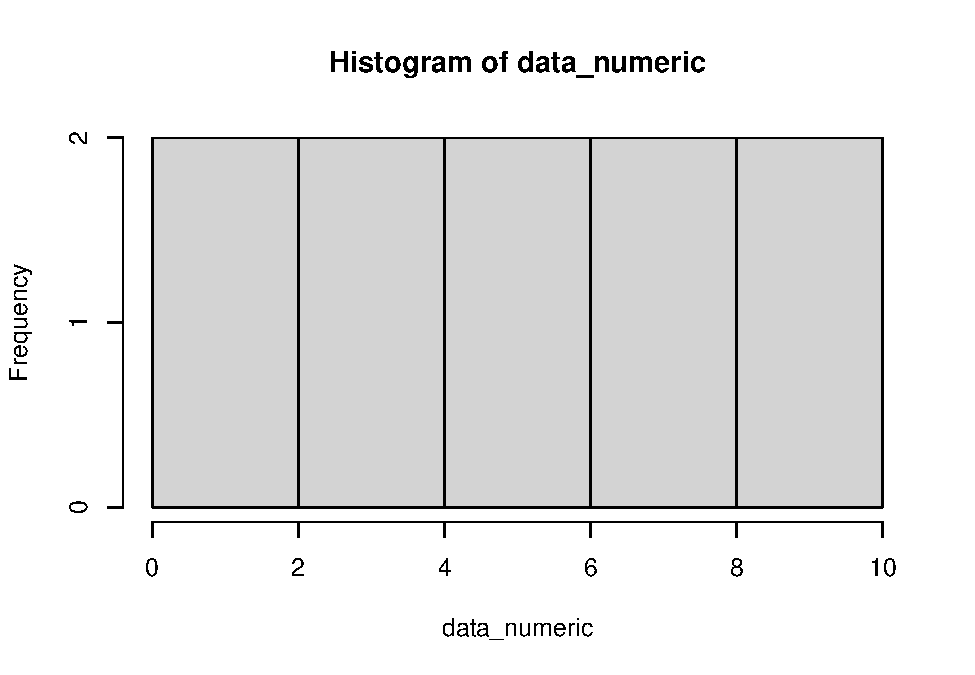
\includegraphics{03-frequencyandplot_files/figure-latex/unnamed-chunk-2-1.pdf}

\hypertarget{bar-graphs}{%
\section{Bar Graphs:}\label{bar-graphs}}

Bar graphs are used for displaying categorical data. Each category is represented by a bar, and the height (or length) of the bar indicates the frequency or count of that category.

\begin{Shaded}
\begin{Highlighting}[]
\CommentTok{\#Bar graph}
\FunctionTok{barplot}\NormalTok{(}\FunctionTok{table}\NormalTok{(data))}
\end{Highlighting}
\end{Shaded}

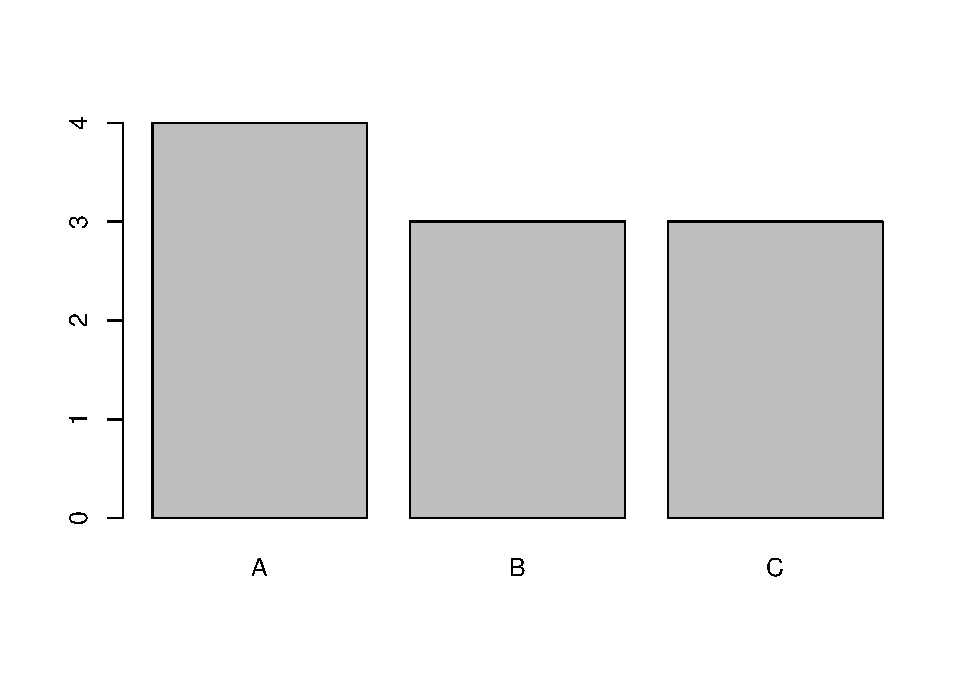
\includegraphics{03-frequencyandplot_files/figure-latex/unnamed-chunk-3-1.pdf}

\hypertarget{pie-charts}{%
\section{Pie Charts:}\label{pie-charts}}

Pie charts represent categorical data as slices of a circle. The size of each slice is proportional to the frequency of each category. Pie charts are useful for visualizing relative proportions of categories.

\begin{Shaded}
\begin{Highlighting}[]
\CommentTok{\#Pie chart}
\FunctionTok{pie}\NormalTok{(}\FunctionTok{table}\NormalTok{(data))}
\end{Highlighting}
\end{Shaded}

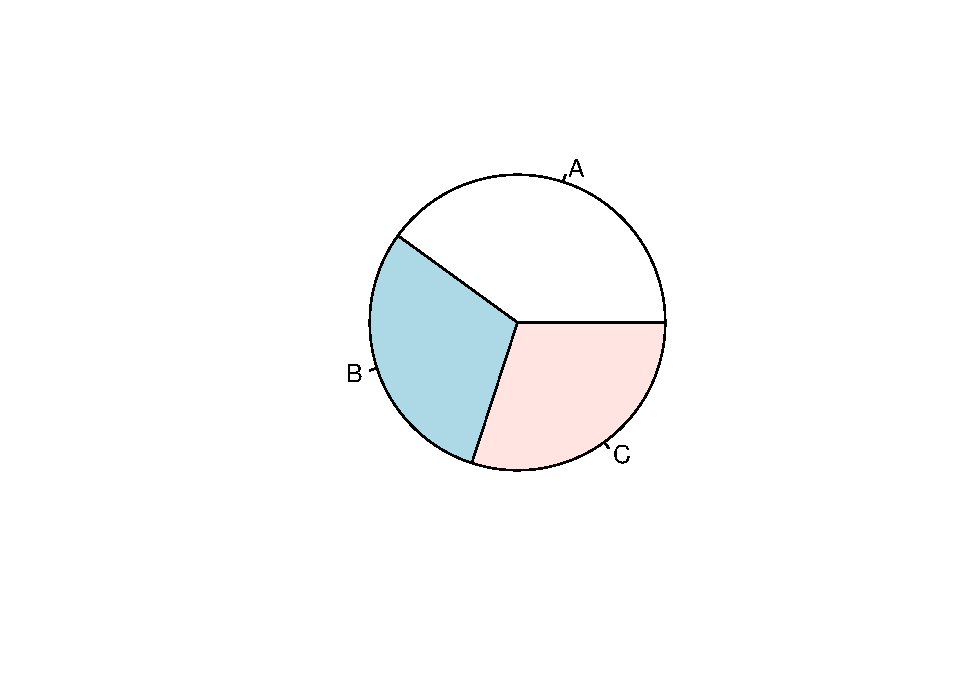
\includegraphics{03-frequencyandplot_files/figure-latex/unnamed-chunk-4-1.pdf}

\hypertarget{box-plots}{%
\section{Box Plots:}\label{box-plots}}

Box plots are used for visualizing the distribution of continuous or discrete numerical data. They show the median, quartiles, and outliers of the data, providing a compact and informative representation of the data distribution.

\begin{Shaded}
\begin{Highlighting}[]
\FunctionTok{boxplot}\NormalTok{(data\_numeric)}
\end{Highlighting}
\end{Shaded}

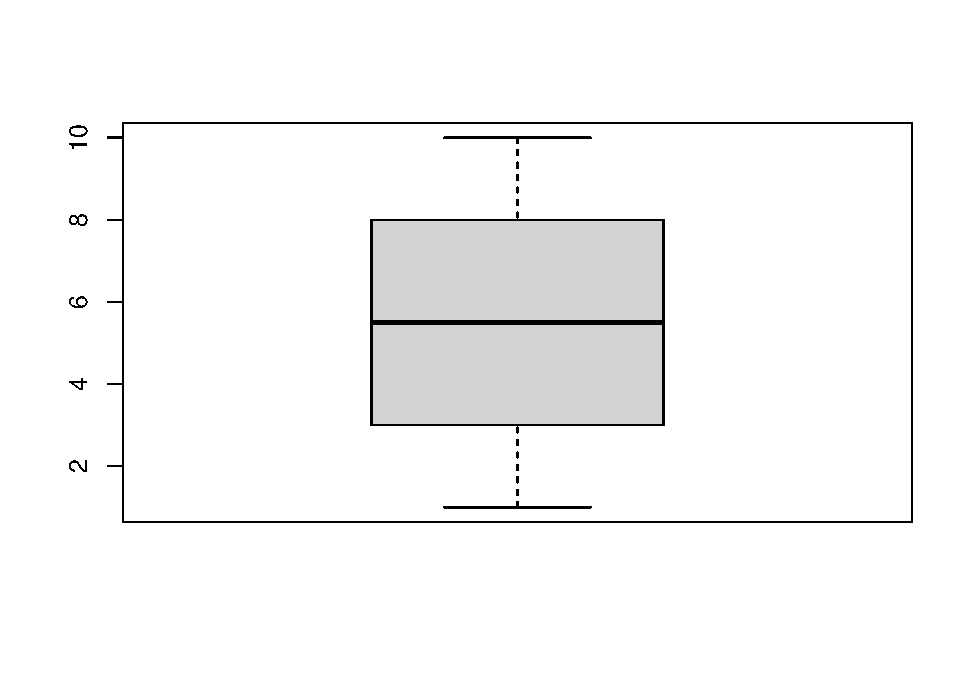
\includegraphics{03-frequencyandplot_files/figure-latex/unnamed-chunk-5-1.pdf}

Each of these data representation techniques serves a different purpose and is suited for different types of data. By understanding when to use each method, you can effectively communicate your data insights and findings.

\hypertarget{describing-data-in-r}{%
\chapter{Describing Data in R}\label{describing-data-in-r}}

\hypertarget{normal-distribution}{%
\chapter{Normal Distribution}\label{normal-distribution}}

\hypertarget{calulate-z-score-using-r}{%
\chapter{Calulate Z-Score using R}\label{calulate-z-score-using-r}}

\hypertarget{computing-z-scores}{%
\chapter{Computing Z-Scores}\label{computing-z-scores}}

\hypertarget{probability-and-inference}{%
\chapter{Probability and Inference}\label{probability-and-inference}}

\#Sampling distribution

\hypertarget{point-estimate}{%
\section{Point Estimate}\label{point-estimate}}

\hypertarget{confidence-interval}{%
\section{Confidence Interval}\label{confidence-interval}}

\hypertarget{hypothesis-signifance-testing}{%
\chapter{Hypothesis Signifance Testing}\label{hypothesis-signifance-testing}}

\#Covariance

\hypertarget{correlation}{%
\chapter{Correlation}\label{correlation}}

\hypertarget{simple-linear-regression}{%
\chapter{Simple Linear Regression}\label{simple-linear-regression}}

\hypertarget{multiple-regression}{%
\chapter{Multiple Regression}\label{multiple-regression}}

\hypertarget{one-way-anova}{%
\chapter{One way ANOVA}\label{one-way-anova}}

\hypertarget{tukeys-post-hoc-tests}{%
\chapter{Tukey's post hoc tests}\label{tukeys-post-hoc-tests}}

\hypertarget{chi-square-tests}{%
\chapter{Chi Square Tests}\label{chi-square-tests}}

\hypertarget{chi-square-goodness-of-fit-test}{%
\section{Chi Square Goodness of Fit Test}\label{chi-square-goodness-of-fit-test}}

\hypertarget{chi-sqaure-test-of-association}{%
\section{Chi Sqaure test of association}\label{chi-sqaure-test-of-association}}

\hypertarget{g-power}{%
\chapter{G* Power}\label{g-power}}

  \bibliography{book.bib}

\end{document}
